\chapter{Practice Exam 3}
    Barry the Biologist has asked for your help to build an amplifier and filter to take small signals
    from his bird sensing microphones and amplify them so that he can capture the signals on his
    PC. The microphone produces AC signals at varying frequencies with 10 mV magnitude. His PC
    requires the signals to be 1 V magnitude. The signals that Barry is interested in are above 1 kHz
    Hz. He would like the filter to attenuate signals at frequencies below 1 kHz. The amplifier and
    filter circuit is to be powered from an AC plugpack. The AC plugpack provides 12 VAC RMS at
    50 Hz.
    \begin{figure}[H]
        \centering
        \includegraphics[width=0.6\linewidth]{figures/exams/ac_plugpack.png}
    \end{figure}
    \begin{enumerate}
        \item Design the power supply component of your amplifier and filter. You will need to
        produce a dual-sided power supply with +10V, 0V and -10V using the 12 VAC plug-
        pack as an AC source. Assume that your amplifier and filter will draw around 10 mA of
        current on both the positive and negative voltage supplies. Your design should include
        components to minimise voltage ripple. Show calculations for the selection of
        components where practical. Show a circuit diagram for the complete power supply
        circuit.\\
        \textbf{Solution:}
        In order to minimise voltage ripple, and to have seperate positive and negative voltage components
        we must use 2 half wave rectifiers and a voltage regulator. The voltage regulator will be used to
        regulate the voltage to 10V. The half wave rectifiers will be used to convert the AC voltage to DC.\\
        \textbf{Calculate the capacitance required for the voltage regulator:}
        \begin{flalign*}
            \Delta v = \frac{1}{fC} \Rightarrow C &= \frac{i}{f\Delta v}\\
            \intertext{Using diodes with a forward voltage of 0.7V, with input voltage of 12RMS ($12\sqrt{2}$ VAC) at 50Hz, current of 10mA, and output voltage of 10V:}
            C &= \frac{10\times 10^{-3}}{50\times \left(12\sqrt{2} - 0.7 - (2+10)\right)} \tag{+2 regulated output voltage for linear regulator}\\
            C &= 47\mu \text{F}
        \end{flalign*}
        \textbf{Positive voltage regulator:}
            \begin{figure}[H]
                \centering
                \begin{circuitikz}[american]
                    \draw (8,2) to [short] (8,0);
                    \draw (0,0) 
                    to[sinusoidal voltage source, v<=12V RMS] (0,2)
                    to [diode, l=0.7V] (4,2)
                    to [short] (6,2)
                    to node[rectangle, draw, fill=white] {LM7810} (10,2)
                    to [short] (12,2);
                    \draw (0,0)
                    to [short] (12,0);
                    % components
                    \draw (4,2) to [capacitor, C=47$\mu$F, *-*] (4,0);
                    \draw (6,2) to [capacitor, C=0.33$\mu$F, *-*] (6,0);
                    \draw (10,2) to [capacitor, C=0.1$\mu$F, *-*] (10,0);
                    \node[right] at (12,1) {$v_{out} = 10$ V};
                    % arrow plus minus at 10
                    \draw[->] (12,1.2) -- (12,2);
                    \draw[->] (12,0.8) -- (12,0);
                \end{circuitikz}
            \end{figure}
        \textbf{Negative voltage regulator}
            \begin{figure}[H]
                \centering
                \begin{circuitikz}[american]
                    \draw (8,2) to [short] (8,0);
                    \draw (0,0) 
                    to[sinusoidal voltage source, v<=12V RMS] (0,2)
                    to [diode, l=0.7V, invert] (4,2)
                    to [short] (6,2)
                    to [short] (12,2);
                    \draw (0,0)
                    to [short] (4,0)
                    to [short] (6,0)
                    to node[rectangle, draw, fill=white] {LM7910} (10,0)
                    to [short] (12,0);
                    % components
                    \draw (4,2) to [capacitor, C=47$\mu$F, *-*] (4,0);
                    \draw (6,2) to [capacitor, C=0.33$\mu$F, *-*] (6,0);
                    \draw (10,2) to [capacitor, C=0.1$\mu$F, *-*] (10,0);
                    \node[right] at (12,1) {$v_{out} = -10$ V};
                    % arrow plus minus at 10
                    \draw[->] (12,1.2) -- (12,2);
                    \draw[->] (12,0.8) -- (12,0);
                \end{circuitikz}
            \end{figure}
        \textbf{Half wave rectifier with positive and negative output}
            \begin{figure}[H]
                \centering
                \begin{circuitikz}[american]
                    \draw (8,2) to [short] (8,0);
                    \draw (0,0)
                        to [sinusoidal voltage source, v<=12V RMS] (0,2)
                        to [short, -*] (1,2)
                        to [diode, l=0.7V] (4,2)
                        to [short, -*] (6,2)
                        to node[rectangle, draw, fill=white] {LM7810} (10,2)
                        to [short] (12,2);
                    \draw (0,0)
                        to [short] (12,0);
                    % components
                    \draw (4,2) to [capacitor, C=47$\mu$F, *-*] (4,0);
                    \draw (6,2) to [capacitor, C=0.33$\mu$F, *-*] (6,0);
                    \draw (10,2) to [capacitor, C=0.1$\mu$F, *-*] (10,0);
                    \node[right] at (12,1) {$v_{out} = 10$ V};
                    % arrow plus minus at 10
                    \draw[->] (12,1.2) -- (12,2);
                    \draw[->] (12,0.8) -- (12,0);
                    % negative part
                    \draw (8,0) to [short, -*] (8,-2);
                    \draw (8,-2) to [short, -*] (8,0);
                    \draw (1,-2)
                        to [diode, l=0.7, invert] (4,-2)
                        to [short, -*] (6,-2)
                        to [short] (12,-2);
                    \draw (4,-2)
                        to [short, -*] (4,-2)
                        to [short, -*] (6,-2)
                        to node[rectangle, draw, fill=white] {LM7910} (10,-2)
                        to [short] (12,-2);
                    % components
                    \draw (4,0) to [capacitor, C=47$\mu$F, *-*] (4,-2);
                    \draw (6,0) to [capacitor, C=0.33$\mu$F, *-*] (6,-2);
                    \draw (10,0) to [capacitor, C=0.1$\mu$F, *-*] (10,-2);
                    \node[right] at (12,-1) {$v_{out} = -10$ V};
                    % arrow plus minus at 10
                    \draw[->] (12,-0.8) -- (12,0);
                    \draw[->] (12,-1.2) -- (12,-2);
                    % connect negative part to voltage source
                    \draw (1,-2) to [crossing] (1,2);
                \end{circuitikz}
            \end{figure}
        \item Design the amplifier and filter circuit to meet Barry’s requirements. The circuit must
        produce the required gain, and also attenuate the signals below 1 kHz. Show calculations
        for the selection of components where practical. Show a circuit diagram for the complete
        amplifier and filter circuit. You do not need to redraw the power supply from part (1)\\
        \textbf{Solution:}
        In order to attenuate signals below 1kHz, and allow signals above 1kHz to pass through, we must
        use a high pass filter with a band pass of 1kHz.\\
        As it needs to amplify signals from 10mV to 1V, the gain must be 100.\\
        \textbf{Active High pass filter:}\\
        \begin{minipage}{0.6\linewidth}
            \begin{figure}[H]
                \begin{circuitikz}[american]
                    \draw (0,0) node[op amp] (opamp) {};
                    \draw (-4.5, 0.5) to [capacitor, l_=159nF] ++(1.5,0);
                    \node[above] at (-5,0.7) {$v_{in}$};
                    \draw (-3,0.5) to[resistor, l=$1\text{k}\Omega$] (opamp.-);
                    \draw (opamp.-) to[short] ++(0,1) to[short] ++(0.5,0) to[resistor, l=$100\text{k}\Omega$] ++(3,0) to[short] ++(0,-1.5);
                      \draw (opamp.out) to[short] ++(2,0) node[right] {$v_o$};
                    % ground
                    \draw (opamp.+) to[short] ++(-0.5,0) to[short] ++(0,-0.5) node[ground] {};
                \end{circuitikz}
            \end{figure}
        \end{minipage}
        \begin{minipage}{0.3\linewidth}
            \begin{flalign*}
                \left|\text{Gain}\right| = \left|-\frac{R_2}{R_1}\right| &= 100\\
                \text{Let }R_1 &= 1\text{k}\Omega\\
                \therefore R_2 &= 100\text{k}\Omega\\
                C = \frac{1}{2\pi f R_2} = \frac{1}{2\pi \times 1\text{k}\times 1\text{k}} &= 159\text{nF}\\
            \end{flalign*}
        \end{minipage}
        \item Perform frequency response analysis for the amplifier and filter you designed in part (2)
        to calculate the gain in dB and phase in degrees when the microphone sends a signal at
        100 Hz, 1k Hz and 10 kHz\\
        \textbf{Solution:}
        Using the general form for the transfer function of an active high pass filter:
        \begin{flalign*}
            H(\omega) &= -\frac{R_2}{R_1} \frac{j\omega}{j\omega + \frac{1}{R_2C_1}} = -100 \frac{j\omega}{j\omega + \frac{1}{1\times 10^3 \times 159\times 10^{-9}}} = -100\frac{j\omega}{j\omega + 6289.31}
        \end{flalign*}
        Note that angles are shifted to the positive quadrant to simplify plotting (still applies the same phase shift)
        \begin{figure}[H]
            \centering
            \begin{tabular}{cccc}
                \textbf{Frequency} & $\boldsymbol{H(\omega)}$ & \textbf{Gain} & $\boldsymbol{\angle H(\omega)}$ \\
                \toprule
                100Hz & $9.947\angle 84.2949^{\circ}$ & 19.948 & 84.2949\\
                1kHz & $70.68\angle 45.03^{\circ}$ & 36.985 & 45.03\\
                10kHz & $99.5\angle 5.72^{\circ}$ & 39.957 & 5.72\\
                \bottomrule
            \end{tabular}
        \end{figure}
        \item Plot the response calculated in part (3) in a Bode plot.\\
            \textbf{Solution:}
            \begin{figure}[H]
                \begin{subfigure}{0.5\textwidth}
                    \centering
                    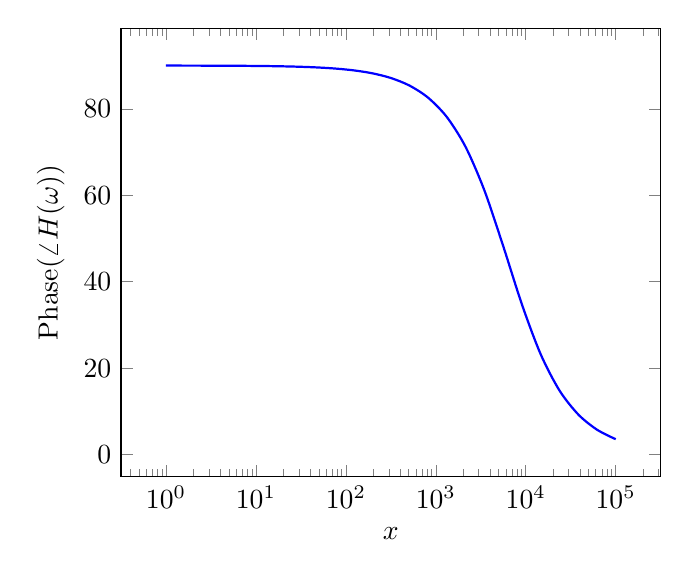
\begin{tikzpicture}
                        \begin{axis}[
                            xlabel=$x$,
                            ylabel=Phase$(\angle H(\omega))$,
                            domain=1:100000,
                            xmode=log,  % Set x-axis to logarithmic scale
                        ]
            
                        \addplot[blue, smooth, thick] {(atan(-x/6289.31))+90};
                        \end{axis}
                    \end{tikzpicture}
                    \caption{Phase plot}
                \end{subfigure}
                \begin{subfigure}{0.5\textwidth}
                    \centering
                    \begin{tikzpicture}
                        \begin{axis}[
                            xlabel=$x$,
                            ylabel=Gain(dB),
                            domain=1:100000,
                            xmode=log,
                        ]
                        \newcommand{\bodemag}{20*log10(sqrt(100 * x^2 / (x^2 + 6289.31^2)))}
                        \addplot[red, domain=1:100000, samples=1000] {\bodemag};
                        \end{axis}
                    \end{tikzpicture}
                    \caption{Magnitude plot}
                \end{subfigure}
                \caption{Phase and Magnitude plots}
            \end{figure}
    \end{enumerate}